\documentclass[onecolumn,11pt,journal]{IEEEtran}
% Phase 2 report: PM2.5 Forecasting with an LSTM and an XGBoost-LSTM Hybrid (Project 19).
% Compile:  tectonic phase2.tex   (or: pdflatex phase2 && bibtex phase2 && pdflatex phase2 && pdflatex phase2)
% Figures are read from ../results/figures/ (generated by the notebooks).
% Every number in this report is taken from results/metrics/ and results/predictions/.

\usepackage[T1]{fontenc}
\usepackage{amsmath,amssymb}
\usepackage{newtxtext,newtxmath}   % professional Times-style text and math fonts
\usepackage{graphicx}
\usepackage{booktabs}
\usepackage{siunitx}
\usepackage{microtype}
\usepackage{cite}
\usepackage{url}
\graphicspath{{../results/figures/}}
\sisetup{detect-all}
\newcommand{\ugm}{\si{\micro\gram\per\cubic\metre}}
\renewcommand{\arraystretch}{1.25}  % a little more breathing room in tables
\linespread{1.1}

\begin{document}

\title{One-Hour-Ahead PM2.5 Forecasting with an LSTM and an XGBoost--LSTM Hybrid}

\author{%
\IEEEauthorblockN{Animesh Kumar Rai \quad Rishiwant Kumar Maurya \quad Supreet \quad Aditya Shankar \quad Drishti Jha}\\[3pt]
\IEEEauthorblockA{Team T051 --- Advance Machine Learning (Phase 2)\\[2pt]
Roll numbers: 2401010069, \ 2401020102, \ 2401010465, \ 2401010038, \ 2401010162}}

\maketitle

\begin{abstract}
This is the Phase~2 (deep learning) report for our Beijing PM2.5 forecasting project. In Phase~1 a feature-engineered XGBoost model beat naive baselines at predicting PM2.5 one hour ahead. Here we ask whether a recurrent neural network, which learns temporal structure directly from the raw hourly history, can match or beat that model, and whether combining the two helps. We train a Long Short-Term Memory (LSTM) network on 24-hour windows of pollution and weather channels, under exactly the same chronological protocol and evaluation hours as Phase~1, so the models are directly comparable. On the 2014 test year the LSTM clearly beats the persistence baseline (MAE 11.28 versus 11.93~\ugm{}, RMSE 20.49 versus 22.03~\ugm{}) and the difference is statistically significant, but it does not beat the tuned XGBoost (MAE 10.96, RMSE 19.96~\ugm{}). Because the two models make partly different errors (their validation errors correlate at 0.95, not 1.0), we form a simple convex blend whose single weight is fixed on 2013 and frozen for 2014. The hybrid gives the best overall test scores (MAE 10.90~\ugm{}, RMSE 19.89~\ugm{}, $R^2$ 0.955) and improves most at high pollution, although its edge over XGBoost alone is small and not statistically significant. We report these results honestly, including where deep learning did not help.
\end{abstract}

\begin{IEEEkeywords}
PM2.5, air quality forecasting, deep learning, LSTM, recurrent neural network, hybrid model, gradient boosting, chronological validation.
\end{IEEEkeywords}

%=====================================================================
\section{Introduction}
Fine particulate matter (PM2.5) is a major health hazard, and short-term forecasts give people and authorities time to respond. In Phase~1 of this project we studied a focused version of the task: \emph{given the pollution and weather observed up to the current hour, predict the PM2.5 concentration one hour later}. We built 37 hand-crafted features from the past and trained an XGBoost model, which reduced the 2014 test error by about 8--9\% over the persistence baseline (carrying the current value forward). That improvement was real but modest, because PM2.5 is highly autocorrelated: consecutive hours are correlated at 0.96, so persistence is already a strong forecast.

Phase~2 asks a different question. Instead of telling the model which lags and rolling windows to use, can a \emph{deep learning} model read the raw recent history and learn the useful temporal patterns by itself? The natural choice is the Long Short-Term Memory (LSTM) network \cite{hochreiter1997}, a recurrent model designed to remember information across many time steps, which has been applied to air-pollution forecasting before \cite{li2017lstm}. Our goals in this phase are:
\begin{enumerate}
\item build an LSTM that forecasts the same one-hour-ahead target from fixed windows of raw hourly channels, with proper regularisation;
\item evaluate it under the \emph{identical} chronological protocol and evaluation hours as Phase~1, so the comparison with XGBoost and the baselines is fair;
\item run an ablation over the window length and network size to understand what matters;
\item build and test a \emph{hybrid} that combines the gradient-boosting and deep-learning forecasts, and report honestly whether it adds value.
\end{enumerate}

The main finding is nuanced and worth stating up front: the LSTM is a strong model that beats the naive baselines significantly, but it does \emph{not} beat the carefully engineered XGBoost at this very short horizon. The hybrid is the best single model overall, but only by a small, statistically insignificant margin. We think these honest results are more useful than an inflated claim that deep learning wins.

%=====================================================================
\section{Related Work}
Bai \emph{et al.} \cite{bai2018} review air-pollution forecasting and note that hybrid methods, which combine complementary models, are a common way to improve on any single approach; our hybrid follows this idea. For the models themselves, Li \emph{et al.} \cite{li2017lstm} applied an LSTM to multi-station Beijing air-quality data, and Zhong \emph{et al.} \cite{zhong2021lightgbm} used gradient boosting (LightGBM) for hourly PM2.5 across China; together they motivate comparing a recurrent network against a tree ensemble on this task. The LSTM architecture itself is due to Hochreiter and Schmidhuber \cite{hochreiter1997}, and XGBoost \cite{chen2016xgboost} is the regularised gradient-boosting method we carry over from Phase~1.

On evaluation we follow the same principles as Phase~1. Tashman \cite{tashman2000} and Bergmeir and Ben\'itez \cite{bergmeir2012} warn against random cross-validation for time series and recommend strictly chronological, out-of-sample testing, and Hyndman and Athanasopoulos \cite{hyndman2021fpp3} stress comparing against naive benchmarks. To decide whether two forecasts genuinely differ in accuracy we use the Diebold--Mariano test \cite{diebold1995} with a Newey--West autocorrelation-robust variance \cite{newey1987}. Reusing exactly this protocol is what lets us place the LSTM directly beside the Phase~1 numbers.

%=====================================================================
\section{Data and Forecasting Protocol}
We use the same public UCI Beijing dataset \cite{uci_beijing,liang2015} as Phase~1: 43{,}824 hourly records from 2010 to 2014, with PM2.5 (\ugm{}) at the US Embassy as the target and dew point, temperature, pressure, wind direction and speed, and snow/rain counters as inputs. The raw file is read-only and its SHA-256 checksum is verified on every load. Only PM2.5 has missing values (2{,}067 hours, 4.7\%, in gaps of up to 155 hours).

To keep Phase~2 directly comparable, we reuse the Phase~1 protocol without change:
\begin{itemize}
\item \textbf{Target.} The forecast is issued at the end of hour $t$ and predicts $x_{t+1}$, the PM2.5 one hour later. Inputs use only hours $\le t$ plus calendar facts of $t+1$; no future weather is used.
\item \textbf{Splits by target hour.} Training is 2010--2012, validation is 2013, and testing is 2014, with each sample assigned to the split that contains its target hour, so no training label lies inside the validation or test period.
\item \textbf{Common evaluation set.} Every model is scored on the identical hours where the target and both baseline inputs are observed: 23{,}452 training, 8{,}563 validation, and 8{,}531 test hours. These are exactly the hours used in Phase~1.
\end{itemize}

%=====================================================================
\section{Input Sequences for the LSTM}
Unlike the tree model, the LSTM is not given hand-made lag and rolling features; it is given the raw recent history and left to learn the temporal structure itself. For each issuance time $t$ we build a window of the previous $L$ hours (hours $t-L+1$ through $t$), with $L$ chosen by the ablation in Section~VII (the selected value is 24~hours). Each hour in the window carries 14 channels: the PM2.5 value, a binary ``was-missing'' flag, dew point, temperature, pressure, the decoded hourly wind speed, a four-way one-hot of the wind direction, the snow and rain counters, and the sine and cosine of the hour of day. This produces an input tensor of shape $43{,}801 \times 24 \times 14$ (samples $\times$ hours $\times$ channels).

Three preprocessing choices matter and all respect the no-leakage rule:
\begin{itemize}
\item \textbf{Missing values.} An LSTM cannot read a NaN, so PM2.5 is forward-filled (the last observed value is carried forward) and the ``was-missing'' flag lets the network discount filled hours; across all windows, 49{,}332 hour-steps are filled. The weather channels have no missing values.
\item \textbf{Scaling.} The continuous channels are standardised to zero mean and unit variance using \emph{training-period statistics only}; validation and test are transformed with those same frozen numbers, so no future information leaks into the scaling.
\item \textbf{Leakage check.} The window for issuance time $t$ ends at hour $t$. We verified this directly: corrupting the PM2.5 value at a future hour $t+1$ leaves every input window unchanged while changing only the target, confirming that no future information enters the inputs. Fig.~\ref{fig:window} shows one example window and the value the model must predict.
\end{itemize}

\begin{figure}[t]
\centering
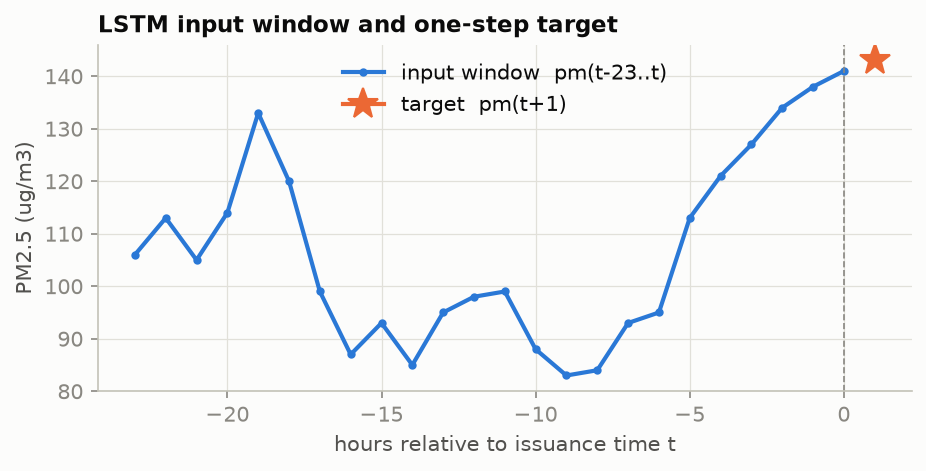
\includegraphics[width=0.72\linewidth]{dl_01_window_example.png}
\caption{One LSTM input: the 24 hours of PM2.5 up to the issuance time $t$ (blue), and the single value at $t+1$ that the network must predict (orange). The dashed line marks $t$; the input never crosses it.}
\label{fig:window}
\end{figure}

%=====================================================================
\section{LSTM Model}
\subsection{Architecture}
The network is a two-layer LSTM with 64 hidden units, followed by a dropout layer and a single linear output. It reads the 24-hour, 14-channel window step by step; the hidden state after the last step (hour $t$) summarises the recent history and is mapped by the linear layer to one number. The selected architecture and training settings are listed in Table~\ref{tab:lstm}.

\subsection{What the network predicts}
As in Phase~1, we found it better to predict the \emph{change} $x_{t+1}-x_t$ and add the current value back, rather than predicting the level $x_{t+1}$ directly. For such a persistent series this gives the network an easier target centred near zero; the learning target is standardised internally for stable training and the transform is inverted at prediction time.

\subsection{Regularisation and training}
Because neural networks can easily overfit, we use several standard safeguards: dropout (rate 0.1), weight decay ($L_2 = 10^{-4}$), and gradient clipping at norm~1.0. Training uses the Adam optimiser (learning rate $10^{-3}$) with a batch size of 256 for up to 40 epochs, and \emph{early stopping}: the most recent 15\% of the training rows are held out, and training stops when their loss stops improving for five epochs. The random seed is fixed. Training ran on an Apple-silicon GPU (Metal/MPS) using PyTorch~2.15; one fit of the selected model takes about 17~seconds. We note that GPU training is not perfectly deterministic, so the reported numbers can vary by a small amount between runs.

\begin{table}[t]
\centering
\caption{Selected LSTM configuration (chosen on the 2013 validation year).}
\label{tab:lstm}
\setlength{\tabcolsep}{8pt}
\begin{tabular}{lc}
\toprule
Setting & Value \\
\midrule
Lookback window & 24 hours \\
LSTM layers & 2 \\
Hidden units & 64 \\
Dropout & 0.1 \\
Prediction target & change ($x_{t+1}-x_t$) \\
Optimiser & Adam, learning rate $10^{-3}$ \\
Weight decay ($L_2$) & $10^{-4}$ \\
Gradient clipping & norm 1.0 \\
Batch size & 256 \\
Max epochs / early-stop patience & 40 / 5 \\
\bottomrule
\end{tabular}
\end{table}

%=====================================================================
\section{Hybrid Model (XGBoost + LSTM)}
A hybrid only helps if its parts make \emph{different} mistakes. On the 2013 validation year the errors of XGBoost and the LSTM are correlated at 0.95 (Fig.~\ref{fig:scatter}): very similar, but not identical, which leaves a little room to gain by combining them. We use the simplest honest combination --- a convex blend of the two forecasts,
\begin{equation}
\hat{y}_{\text{hybrid}} = w\,\hat{y}_{\text{xgb}} + (1-w)\,\hat{y}_{\text{lstm}},
\label{eq:blend}
\end{equation}
with a single weight $w \in [0,1]$. We choose $w$ by least squares on the 2013 validation year and then \emph{freeze} it for the 2014 test, so nothing from the test is used to build the hybrid. The fitted weight is $w = 0.63$ (63\% XGBoost, 37\% LSTM). Using one parameter, tuned on validation only, keeps the hybrid simple and hard to overfit; this is a deliberate choice over a more complex stack of models.

\begin{figure}[t]
\centering
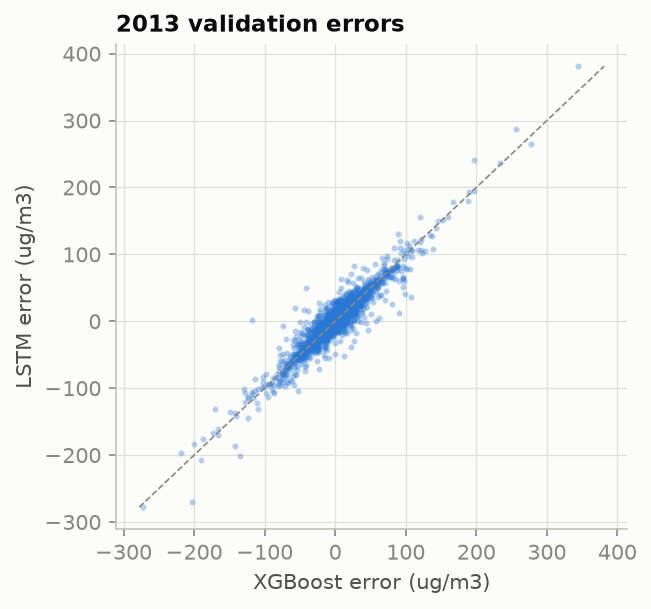
\includegraphics[width=0.52\linewidth]{dl_05_error_scatter.png}
\caption{XGBoost error versus LSTM error on the 2013 validation hours. The errors are strongly correlated (0.95) but not identical, which is why a blend can help a little.}
\label{fig:scatter}
\end{figure}

%=====================================================================
\section{Experimental Setup}
\textbf{Tuning the LSTM.} We tuned three things by grid search --- the lookback window (24, 48, 72 hours), the hidden size (32, 64), and the number of layers (1, 2) --- giving 12 configurations. Each is trained once on 2010--2012 and scored on the 2013 validation hours, and the lowest validation MAE is selected and frozen for the test. Using a single held-out year (rather than Phase~1's four quarterly folds) keeps the deep-learning search affordable; 2013 is never used in training, so the comparison stays leakage-free.

\textbf{Test evaluation.} With the configuration frozen, the LSTM is evaluated on 2014 exactly as XGBoost was: the model is refit before each of the twelve months using all earlier data (an expanding window), and predictions are collected only on the common evaluation hours.

\textbf{Metrics.} We report MAE, RMSE and $R^2$, and use the Diebold--Mariano test (with an autocorrelation-robust variance) to check whether differences between forecasts are statistically significant. A negative Diebold--Mariano statistic means the first model has the lower loss.

%=====================================================================
\section{Results}
\subsection{Tuning and ablation (2013)}
Table~\ref{tab:search} lists all twelve configurations. Every one beats the persistence baseline (MAE 13.18~\ugm{}), so the LSTM reliably learns something useful. The best configuration uses the \emph{shortest} window, 24~hours; longer windows of 48 or 72 hours gave no improvement. This agrees with Phase~1's finding that only the most recent hours carry strong predictive information at this one-hour horizon. Two layers with 64 hidden units was the best size, but the spread across all configurations is small (validation MAE 12.47--12.85~\ugm{}), so the LSTM is not very sensitive to these choices. Fig.~\ref{fig:search} shows the same result graphically.

\begin{table}[t]
\centering
\caption{LSTM tuning on 2013 (all 12 configurations, sorted by validation MAE). MAE and RMSE in \ugm{}.}
\label{tab:search}
\setlength{\tabcolsep}{7pt}
\begin{tabular}{ccccc}
\toprule
Lookback (h) & Hidden & Layers & MAE & RMSE \\
\midrule
\textbf{24} & \textbf{64} & \textbf{2} & \textbf{12.47} & \textbf{22.85} \\
72 & 64 & 1 & 12.52 & 22.86 \\
72 & 64 & 2 & 12.52 & 22.94 \\
48 & 32 & 2 & 12.54 & 23.06 \\
24 & 64 & 1 & 12.59 & 23.05 \\
24 & 32 & 2 & 12.71 & 23.24 \\
72 & 32 & 2 & 12.72 & 23.20 \\
48 & 64 & 2 & 12.74 & 23.18 \\
48 & 64 & 1 & 12.77 & 23.25 \\
24 & 32 & 1 & 12.79 & 23.40 \\
72 & 32 & 1 & 12.80 & 23.32 \\
48 & 32 & 1 & 12.85 & 23.31 \\
\bottomrule
\end{tabular}
\end{table}

\begin{figure}[t]
\centering
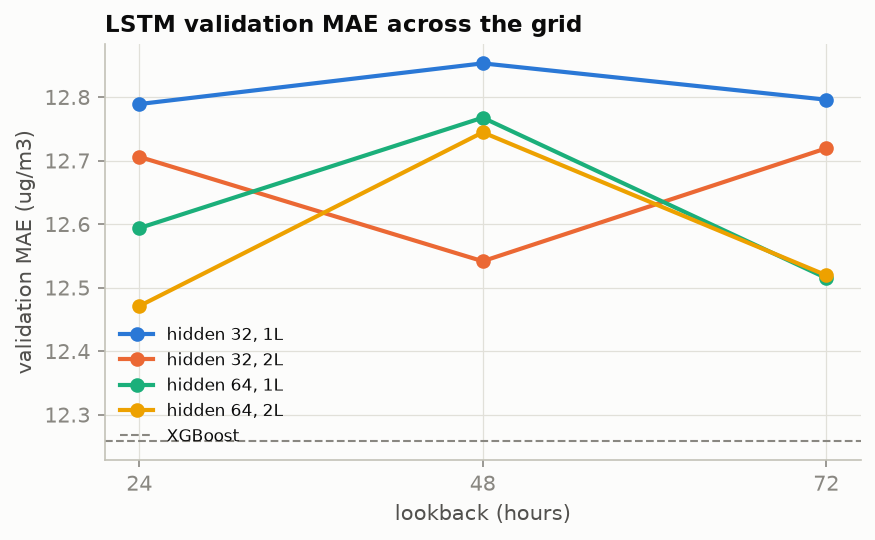
\includegraphics[width=0.74\linewidth]{dl_02_lstm_search.png}
\caption{Validation MAE across the tuning grid. All settings beat persistence; the dashed line is XGBoost (12.26~\ugm{}). The shortest 24-hour window does best.}
\label{fig:search}
\end{figure}

\subsection{Validation comparison (2013)}
Pooled over the 2013 validation hours, the selected LSTM reaches MAE 12.47 and RMSE 22.85~\ugm{} (Table~\ref{tab:val}). This is clearly better than persistence (13.18 / 24.87) but a little behind XGBoost (12.26 / 22.53). In other words, learning the temporal pattern from raw history gets very close to the hand-engineered tree model, but does not overtake it.

\begin{table}[t]
\centering
\caption{Validation results (2013, 8{,}563 common hours). MAE and RMSE in \ugm{}.}
\label{tab:val}
\setlength{\tabcolsep}{8pt}
\begin{tabular}{lccc}
\toprule
Model & MAE & RMSE & $R^2$ \\
\midrule
Persistence & 13.18 & 24.87 & 0.936 \\
XGBoost (change) & 12.26 & 22.53 & 0.947 \\
LSTM & 12.47 & 22.85 & 0.946 \\
\bottomrule
\end{tabular}
\end{table}

\subsection{Test-year results (2014)}
Table~\ref{tab:test} shows the single, final evaluation on 2014. The ordering from validation holds on the test year: the LSTM (MAE 11.28, RMSE 20.49) comfortably beats persistence (11.93, 22.03) --- about a 5\% lower MAE and 7\% lower RMSE --- but stays behind XGBoost (10.96, 19.96). The seasonal-naive baseline again has a negative $R^2$ and is not a useful forecast. The \emph{hybrid} achieves the best scores of any model: MAE 10.90, RMSE 19.89, and the highest $R^2$ (0.955). Fig.~\ref{fig:compare} compares the models, and Fig.~\ref{fig:monthly} shows that the LSTM tracks between persistence and XGBoost in every month of the year, with no month where it collapses.

\begin{table}[t]
\centering
\caption{Test-year results (2014, 8{,}531 common hours). Best value in each column in bold. MAE and RMSE in \ugm{}.}
\label{tab:test}
\setlength{\tabcolsep}{8pt}
\begin{tabular}{lccc}
\toprule
Model & MAE & RMSE & $R^2$ \\
\midrule
Persistence & 11.93 & 22.03 & 0.944 \\
Seasonal-naive (24 h) & 67.30 & 98.75 & $-0.121$ \\
XGBoost (change) & 10.96 & 19.96 & 0.954 \\
LSTM & 11.28 & 20.49 & 0.952 \\
\textbf{Hybrid (0.63 XGB + 0.37 LSTM)} & \textbf{10.90} & \textbf{19.89} & \textbf{0.955} \\
\bottomrule
\end{tabular}
\end{table}

\begin{figure}[t]
\centering
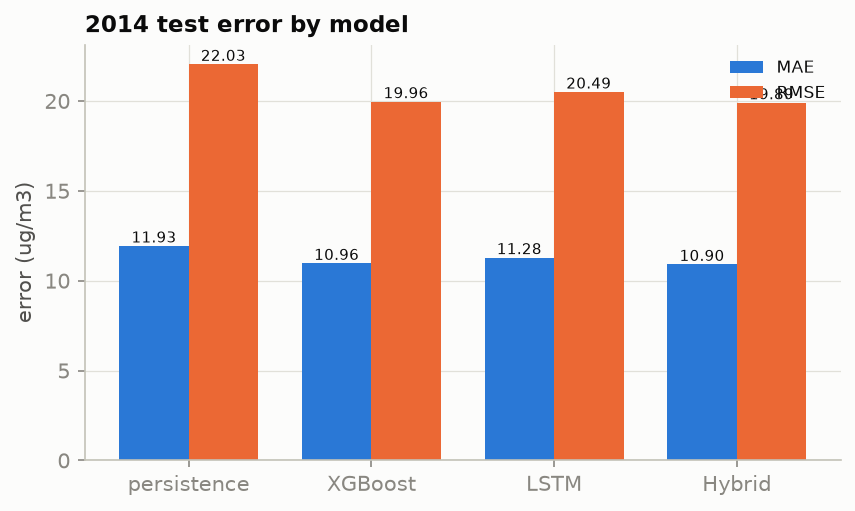
\includegraphics[width=0.74\linewidth]{dl_06_hybrid_compare.png}
\caption{Test-year MAE and RMSE by model. The hybrid is slightly better than XGBoost, which is better than the LSTM, which is better than persistence.}
\label{fig:compare}
\end{figure}

\begin{figure}[t]
\centering
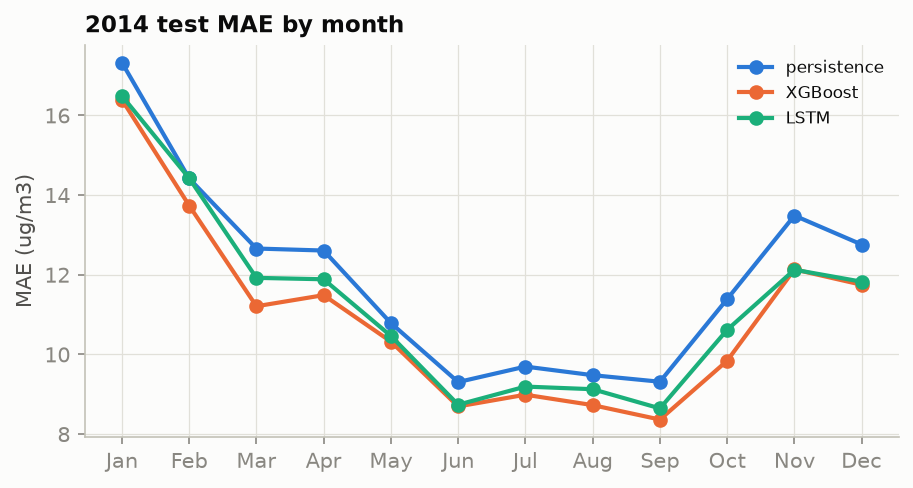
\includegraphics[width=0.8\linewidth]{dl_03_test_monthly.png}
\caption{Monthly test MAE in 2014. The LSTM (green) tracks between persistence (blue) and XGBoost (orange) throughout the year.}
\label{fig:monthly}
\end{figure}

\subsection{Is the difference significant?}
Table~\ref{tab:dm} reports the Diebold--Mariano tests on the 2014 test hours. The LSTM is significantly better than persistence (for example $p \approx 3\times10^{-8}$ on squared-error loss), confirming that the deep model adds genuine skill over carrying the value forward. XGBoost is significantly better than the LSTM ($p \approx 2\times10^{-5}$ on absolute loss), so the tree model's small advantage is real, not noise. The hybrid's improvement over XGBoost, however, is \emph{not} statistically significant ($p = 0.55$ on squared loss, $p = 0.07$ on absolute loss): the blend helps consistently but only by a little, and we do not overstate it.

\begin{table}[t]
\centering
\caption{Diebold--Mariano tests on the 2014 test hours. A negative statistic means the first model has the lower loss.}
\label{tab:dm}
\setlength{\tabcolsep}{7pt}
\begin{tabular}{llcc}
\toprule
Comparison & Loss & DM stat. & $p$-value \\
\midrule
LSTM vs persistence & squared  & $-5.54$ & $3.1\times10^{-8}$ \\
LSTM vs persistence & absolute & $-6.17$ & $6.8\times10^{-10}$ \\
LSTM vs XGBoost     & squared  & $+2.13$ & $0.033$ \\
LSTM vs XGBoost     & absolute & $+4.29$ & $1.8\times10^{-5}$ \\
Hybrid vs XGBoost   & squared  & $-0.60$ & $0.549$ \\
Hybrid vs XGBoost   & absolute & $-1.82$ & $0.069$ \\
\bottomrule
\end{tabular}
\end{table}

\subsection{Error by pollution level}
Grouping the test hours by their true PM2.5 level (Table~\ref{tab:level} and Fig.~\ref{fig:level}) shows where each model helps. The LSTM is slightly worse than XGBoost in the two lowest bands but close to it elsewhere. The hybrid is more interesting: it \emph{improves on XGBoost in the three higher bands} --- 75--150, 150--250, and the extreme band above 250~\ugm{} (MAE 23.53 versus 23.92) --- at the cost of being marginally worse in the two lowest bands. In other words, the LSTM's different errors pull the high-pollution predictions down, and since those hours carry the largest errors, the blend wins overall. That said, no model solves the extreme band: above 250~\ugm{} all three have RMSE near 42~\ugm{} (persistence 41.6, XGBoost 42.0, LSTM 42.2), so the sudden, rare pollution spikes remain the hardest part of the problem --- the same wall Phase~1 hit.

\begin{table}[t]
\centering
\caption{Test MAE (\ugm{}) by true PM2.5 level, with the number of hours in each band.}
\label{tab:level}
\setlength{\tabcolsep}{7pt}
\begin{tabular}{lccccc}
\toprule
Band (\ugm{}) & Hours & Persist. & XGBoost & LSTM & Hybrid \\
\midrule
0--35    & 2485 & 5.64  & \textbf{5.48}  & 5.86  & 5.55 \\
35--75   & 1937 & 10.61 & \textbf{9.39}  & 9.75  & 9.43 \\
75--150  & 2399 & 13.14 & 11.82 & 11.95 & \textbf{11.69} \\
150--250 & 1061 & 18.83 & 16.78 & 17.29 & \textbf{16.62} \\
$>250$   & 649  & 24.18 & 23.92 & 24.28 & \textbf{23.53} \\
\bottomrule
\end{tabular}
\end{table}

\begin{figure}[t]
\centering
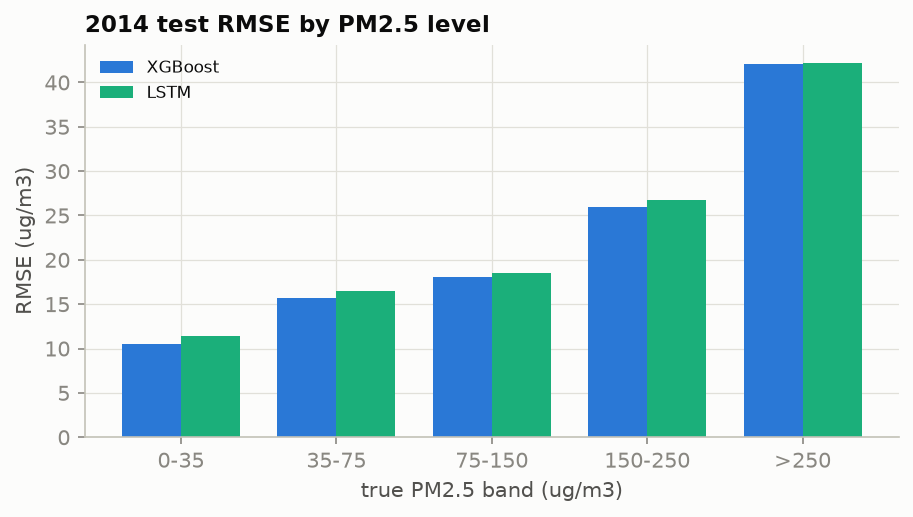
\includegraphics[width=0.72\linewidth]{dl_04_test_by_level.png}
\caption{Test-year RMSE grouped by true PM2.5 level, XGBoost versus LSTM. Both rise sharply in the extreme band; neither solves it.}
\label{fig:level}
\end{figure}

%=====================================================================
\section{Discussion}
Three honest conclusions come out of these experiments. First, the LSTM is a capable model: given only the raw hourly history it learns to beat the naive baselines significantly, and it does so steadily across the whole test year. This shows the deep model can discover the useful temporal structure on its own, without the 37 hand-made features of Phase~1.

Second, learning from raw history did \emph{not} beat careful feature engineering at this horizon. XGBoost remains the stronger single model, and the Diebold--Mariano test confirms its edge is real. This is a reasonable outcome: when the next hour is already 96\% correlated with the current one, the problem is dominated by short-range persistence, which the compact Phase~1 features capture very efficiently; there is simply little long-range structure for a recurrent network to exploit one hour ahead. The ablation supports this --- a longer memory (48 or 72 hours) did not help.

Third, the hybrid is the best model overall, and the reason is instructive: the two models' errors are correlated but not identical, so blending them cancels some error, especially at high pollution where their mistakes differ most. The gain is small and not statistically significant, so we present the hybrid as a modest, well-justified improvement rather than a breakthrough. Crucially, its weight was fixed on validation and frozen for the test, and it still improved the test year, which shows the small gain is a genuine generalisation and not test-set tuning.

%=====================================================================
\section{Limitations and Future Scope}
\textbf{Limitations.} As in Phase~1, the results come from a single monitoring station and a single test year, so the exact numbers should not be over-generalised. The LSTM was trained on a GPU, which is not perfectly deterministic, so its numbers can shift slightly between runs. We tuned the deep model on a single validation year rather than multiple folds, to keep training affordable. No model improves on the extreme pollution hours, and the hybrid's advantage over XGBoost is not statistically significant.

\textbf{Future scope.} Several directions could extend this phase: a temporal convolutional network as an alternative deep model; a loss function that weights the rare extreme hours more heavily, which is where every model struggles; adding operational weather forecasts as inputs so the models can anticipate sudden build-ups; and mapping the forecast to standard AQI categories for a more user-facing output. A more thorough but costlier evaluation would retune the LSTM with the same multi-fold scheme used for XGBoost.

%=====================================================================
\section{Conclusion}
In Phase~2 we built and evaluated an LSTM for one-hour-ahead Beijing PM2.5 forecasting, under exactly the same leakage-controlled, chronological protocol as the Phase~1 machine learning work. The LSTM learns useful temporal structure directly from raw hourly channels and significantly beats the naive baselines (test MAE 11.28 versus 11.93~\ugm{}), but it does not overtake the feature-engineered XGBoost (10.96~\ugm{}). A simple convex hybrid of the two, with its single weight fixed on validation and frozen for the test, gives the best overall test scores (MAE 10.90~\ugm{}, $R^2$ 0.955) and helps most at high pollution, though its edge over XGBoost alone is small and not significant. Beyond the numbers, the project shows sound deep-learning practice on time-series data --- windowed inputs with no leakage, training-only scaling, proper regularisation, a fair comparison against a strong prior model, and an honest account of where deep learning did and did not help. All results are reproducible from the project notebooks.

\bibliographystyle{IEEEtran}
\bibliography{references}

\end{document}
